% ============================================================
%  Generating Synthetic FMCW Radar Data for Evaluating
%  Visual Docking Guidance Systems in Low Visibility
%  Author: Kashan Haider
%
%  Every number in Section VI comes from the open implementation:
%  experiments/run_m1.py (results_m1.json) and
%  experiments/run_all.py (results_all.json), seed 2026.
% ============================================================
\documentclass[conference]{IEEEtran}
\IEEEoverridecommandlockouts

% ---------- Packages ----------
\usepackage[utf8]{inputenc}
\usepackage[T1]{fontenc}
\usepackage{cite}
\usepackage{amsmath,amssymb,amsfonts}
\usepackage{graphicx}
\usepackage{booktabs}
\usepackage{multirow}
\usepackage{siunitx}
\usepackage{xcolor}
\usepackage{listings}
\usepackage[hidelinks]{hyperref}
\usepackage[capitalise,noabbrev]{cleveref}

\graphicspath{{figures/}}
\sisetup{detect-all, retain-explicit-plus}

\lstset{
  basicstyle=\ttfamily\scriptsize,
  breaklines=true,
  frame=single,
  columns=fullflexible
}

% ---------- Title and author ----------
\title{Generating Synthetic FMCW Radar Data for Evaluating Visual Docking Guidance Systems in Low Visibility}

\author{
  \IEEEauthorblockN{Kashan Haider}
  \IEEEauthorblockA{\textit{Master System Integration} \\
  \textit{Source Integreta}\\
  Noida, India \\
  kashan@sourceintegreta.com}
}

\begin{document}

\maketitle

% ============================================================
\begin{abstract}
Visual Docking Guidance Systems (VDGS) guide aircraft to the stop position at the gate. Their laser and camera sensors lose range in fog, so manufacturers are adding radar. Validating a radar-augmented VDGS normally requires trials on the apron, which are costly, weather-dependent and hard to repeat. Earlier work emulated undocumented radar files by brute-force byte search and needed 42{,}218 attempts to produce one detection at one fixed range. This paper presents an open, software-only framework that generates synthetic frequency-modulated continuous-wave (FMCW) radar data from the beat-frequency and Doppler relations of the radar, and carries it through detection, a reference docking logic and the hand-off of on-block events to airport operations. Any commanded range is produced in one generation: across 1{,}101 ranges from \SIrange{5}{60}{\metre}, the recovered range had an RMSE of \SI{0.34}{\centi\metre} against a \SI{30}{\centi\metre} range bin. On a catalogue of 13 scenarios, the nominal docking reported the Actual In-Block Time (AIBT) within \SI{0.17}{\second} and the stop position within \SI{1.4}{\centi\metre} over 20 runs. Fault injection showed that a \SI{2}{\second} loss of the detection stream suppressed the AIBT entirely while every sensor-level check still passed. The framework exposed four failures in a first version of the docking logic; three were fixed and confirmed by regression tests, and one, a stationary ghost echo near the stop line, remains open. The full pipeline ran at \SI{14}{\milli\second} per frame against a \SI{200}{\milli\second} budget.
\end{abstract}

\begin{IEEEkeywords}
FMCW radar, synthetic data, visual docking guidance system, airport operations, low visibility, fault injection, A-CDM
\end{IEEEkeywords}

% ============================================================
\section{Introduction}
\label{sec:intro}

At a contact stand, the last metres of an aircraft's taxi are guided by a Visual Docking Guidance System (VDGS) mounted on the terminal wall. It measures the approaching aircraft and tells the pilot how far it is to the stop position and whether it is on the centreline \cite{us6762694}. The same system also reports when the aircraft is on block. That time stamp, the Actual In-Block Time (AIBT), is one of the milestones of Airport Collaborative Decision Making (A-CDM) and drives the planning of the turnaround that follows \cite{icao_acdm,caas_acdm}.

Most installed systems measure the aircraft with a scanning laser. Its range is typically \SIrange{100}{200}{\metre} in good weather and shrinks in fog, rain and snow \cite{us10384805}. Radar is far less affected, which is why radar is being added to VDGS designs, alone or fused with other sensors \cite{us11756440}. Adding a sensor, however, raises a testing problem. Low-visibility conditions cannot be ordered on demand, apron time is scarce, and a failed trial cannot be repeated exactly. Faults that matter are also not limited to the sensor: a delayed or lost detection message can corrupt the AIBT that leaves the VDGS, even when the radar itself is working.

The closest prior work tried to emulate radar input for a commercial radar-augmented VDGS without a format specification \cite{khalil2020radar}. It recovered the outer layout of the recorded files but not the meaning of the sample data, and fell back on trial and error. Producing one file that the vendor software detected at \SI{21}{\metre} took 42{,}218 attempts. The result covered one static range, gave no control over target speed or number, and could only be checked with closed vendor software. Automotive research offers mature radar models for virtual testing \cite{magosi2022survey}, but they stop at the sensor and do not address docking geometry or the airport systems a VDGS feeds.

This paper replaces byte-level search with a physical signal model and extends the test chain to airport operations. The framework computes radar baseband samples from the FMCW beat-frequency and Doppler relations, processes them with an open reference processor, sends detections as JSON over UDP to a reference docking logic, and passes the resulting events to a mock airport operational database (AODB) that computes the target off-block time. Faults can be injected on the radar side and on the detection stream. The work followed an iterative design-and-evaluate cycle \cite{peffers2007dsr}, and the results reported here include the failures that the cycle exposed.

The paper addresses three research questions:
\begin{itemize}
  \item \textbf{RQ1}: Can a physics-based model generate radar data that yields correct detections at any commanded range, without search?
  \item \textbf{RQ2}: Can the same model reproduce dynamic docking scenarios, including stops, overshoots and obstacles, at the \SI{5}{\hertz} update rate of a radar VDGS?
  \item \textbf{RQ3}: Does end-to-end simulation reveal faults that sensor-level checks miss?
\end{itemize}

The contributions are:
\begin{itemize}
  \item a physics-based generator of synthetic FMCW radar data for apron docking, with an extended aircraft target model;
  \item a five-layer framework that carries the generated data through detection, the VDGS interface and docking logic, and the hand-off of AIBT and AOBT to a mock AODB;
  \item a catalogue of 13 scenarios with fixed acceptance criteria, covering static ranges, dynamic dockings, obstacles, degraded signal-to-noise ratio and stream faults;
  \item an evaluation against the brute-force baseline, and a record of four docking-logic failures found by the framework, three of them fixed and regression-tested;
  \item an open implementation in which every reported number is regenerated by a script with a fixed random seed.
\end{itemize}

\Cref{sec:background} introduces FMCW radar and docking operations, \cref{sec:related} reviews related work, \cref{sec:framework} presents the framework and \cref{sec:implementation} its implementation. \Cref{sec:evaluation} reports the results, \cref{sec:discussion} discusses them and their limits, and \cref{sec:conclusion} concludes.

% ============================================================
\section{Background}
\label{sec:background}

\subsection{FMCW Radar Principles}
An FMCW radar transmits a sequence of chirps, signals whose frequency rises linearly over a bandwidth $B$ during a ramp time $T_c$, giving a slope $S = B/T_c$ \cite{rao_ti_fmcw}. The receiver mixes the echo with the chirp being transmitted. Because the echo from a target at range $R$ arrives after a round-trip delay of $2R/c$, the mixer output is a tone at the beat frequency
\begin{equation}
  f_b = \frac{2 S R}{c},
  \label{eq:beat}
\end{equation}
where $c$ is the speed of light. Range estimation therefore reduces to frequency estimation, done with a fast-time FFT over the $N_s$ samples of each chirp. Two targets are separated if their beat frequencies differ by at least one FFT bin, which gives the range resolution
\begin{equation}
  \Delta R = \frac{c}{2B}.
  \label{eq:rres}
\end{equation}
With complex (I/Q) sampling at rate $f_s$, beat frequencies up to $f_s$ are unambiguous, so the maximum range is $R_{\max} = f_s c / (2S)$.

A target moving with radial velocity $v$ changes the echo phase between consecutive chirps by
\begin{equation}
  \Delta\phi = \frac{4\pi v T_c}{\lambda},
  \label{eq:doppler}
\end{equation}
where $\lambda$ is the carrier wavelength. A slow-time FFT across the $N_c$ chirps of a frame measures this phase rate and hence the speed. The largest unambiguous speed is $v_{\max} = \lambda/(4T_c)$ and the speed resolution is $\Delta v = \lambda/(2 N_c T_c)$.

\subsection{Docking Guidance and Airport Operations}
A VDGS tracks the aircraft from stand entry to the stop position and shows the pilot the remaining distance and any lateral deviation \cite{us6762694}. Its outputs also feed airport systems. When the aircraft comes to rest at the stand, the docking system is a typical source of the AIBT \cite{icao_acdm,schiphol_acdm}. Later A-CDM milestones build on it. At Singapore Changi, for example, the system target off-block time (TOBT) is the AIBT plus the minimum turnaround time (MTT), or the scheduled departure time if that is later \cite{caas_acdm}. A wrong, late or missing AIBT therefore propagates into turnaround planning, not only to the pilot display.

% ============================================================
\section{Related Work}
\label{sec:related}

\subsection{Radar Data Emulation for Docking Systems}
Khalil and Hojeij tried to emulate the input of a commercial radar VDGS \cite{khalil2020radar}. They received 2{,}764 recorded radar files of \num{3154944} bytes each, without a format specification. By inspecting the files they recovered the outer structure: a file-start token, 512 chirps of \num{6162} bytes, and an 18-byte header per chirp holding a chirp-start token, a file counter and a byte counter. They could not relate the remaining \num{6144} bytes per chirp to the target, and fell back on trial and error. After 60{,}000 generated files, attempt 42{,}218 produced detections from \SIrange{21}{28}{\metre}, meeting the client's requirement of a detection beyond \SI{21}{\metre}. The approach covered one static range and depended on the vendor's closed processing software. The present work keeps the requirements the authors recorded, namely detections beyond \SI{21}{\metre}, five scans per second and a JSON detection format, but replaces the search with a physical model.

\subsection{Radar Sensor Models for Virtual Validation}
Radar simulation for virtual testing is most developed in the automotive domain. Magosi et al.\ survey the field and classify sensor models by their role in the V-model into operational, functional, technical and individual models \cite{magosi2022survey}. Measurement studies show why high-fidelity radar models remain hard: multipath propagation, the separability of close targets, and the sensitivity of radar cross-section (RCS) to aspect angle \cite{holder2018challenges}. Sensitivity analysis has been proposed to decide how much model detail a given test needs \cite{ngo2020sensitivity}, and physical radar simulation has been scaled to interacting digital twins \cite{thieling2021scalable}. Open tools such as RadarSimPy generate baseband data from point targets and ray-traced scenes \cite{radarsimpy}. This work adopts the same physical relations at a deliberately low level of fidelity, and applies them to a setting the automotive models do not cover: apron docking geometry and the hand-off from the docking system to airport operations.

\subsection{Airport Systems and A-CDM}
A-CDM documents define the milestones, their sources and how later targets are derived \cite{icao_acdm,schiphol_acdm,caas_acdm}. They treat the docking system as a data source and assume its output is correct. VDGS literature consists mainly of patents on sensing, range and display \cite{us6762694,us10384805,us11756440}. To the author's knowledge, no published work tests the chain from radar data to A-CDM milestones as one system.

% ============================================================
\section{Proposed Framework}
\label{sec:framework}

\subsection{Overview}
\Cref{fig:arch} shows the five layers. A scenario defines what happens on the stand and provides ground truth at the \SI{5}{\hertz} frame rate. The radar data layer turns the scene into complex baseband samples. The reference processor turns samples into detections. The VDGS layer receives detections as JSON over UDP, tracks the aircraft and raises docking events. The integration layer passes events to a mock AODB. A fault injector acts on the radar data and on the detection stream, and an evaluator compares every layer's output with the scenario truth.

\begin{figure}[t]
  \centering
  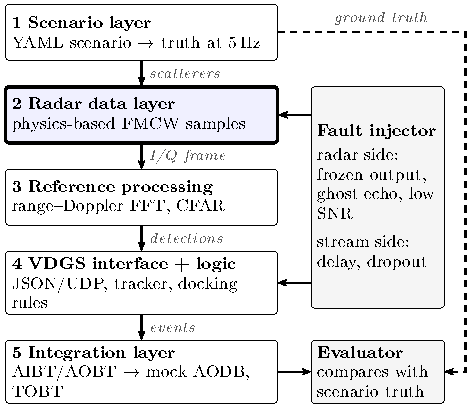
\includegraphics[width=\linewidth]{architecture.pdf}
  \caption{Framework architecture. The radar data layer (bold) replaces byte-level emulation; layers 3 to 5 make the evaluation end to end.}
  \label{fig:arch}
\end{figure}

\subsection{Scenario Layer}
The radar sits on the terminal wall on the stand centreline, and range is measured along that line. Each scenario is a YAML file that sets the aircraft trajectory, other actors, static reflectors, the signal-to-noise ratio and any faults. The aircraft enters at a constant speed, brakes at a constant deceleration and stops at the stop line plus an optional stop error; it may later push back. Vehicles and people cross the stand at a perpendicular distance $d$ from the wall. An actor at lateral position $x$ has range $\sqrt{d^2+x^2}$ and radial speed $x v_x/\sqrt{d^2+x^2}$, and is seen only inside a \SI{60}{\degree} field of view. Ground truth, including the true stop time, comes from the same closed-form trajectory.

\subsection{Radar Data Layer}
\label{sec:radar-layer}
The radar data layer models the radar after dechirping, so it never needs the transmitted waveform at radio frequency. Each scatterer $i$ has range $R_i$, radial velocity $v_i$ and amplitude $a_i$. Sample $n$ of chirp $k$ is
\begin{equation}
  x[k,n] = \sum_i a_i \, e^{\,j\left(2\pi f_{b,i} n / f_s \;+\; 4\pi R_i/\lambda \;+\; k\,\Delta\phi_i\right)} + w[k,n],
  \label{eq:signal}
\end{equation}
where $f_{b,i}$ follows \cref{eq:beat}, $\Delta\phi_i$ follows \cref{eq:doppler}, and the middle term is the carrier phase of the round trip. The amplitude follows the radar equation, $a_i = \sqrt{\sigma_i}\,(R_\text{ref}/R_i)^2$, so received power falls with $\sigma_i/R_i^4$ for an RCS $\sigma_i$. A \SI{1}{\square\metre} scatterer at $R_\text{ref} = \SI{20}{\metre}$ has unit amplitude. The noise $w[k,n]$ is circular complex Gaussian, and its level is set by the reference SNR: the per-sample SNR of that reference scatterer.

\Cref{eq:signal} is the key difference from byte-level emulation \cite{khalil2020radar}. Range, speed and RCS are inputs to a closed-form expression, so a frame for any scene is produced directly instead of being searched for.

An aircraft seen nose-on is not a point. It is modelled as three scattering centres: the nose (\SI{10}{\square\metre}), the nose gear \SI{5}{\metre} behind it (\SI{3}{\square\metre}) and the engine inlets \SI{11.5}{\metre} behind it (\SI{30}{\square\metre}). These values are illustrative simulation inputs, not measured signatures. They matter because the nose, which the VDGS must track, is weaker than the engines behind it.

\Cref{tab:params} lists the radar parameters. They are design choices for the simulation, not those of a commercial product. A \SI{500}{\mega\hertz} bandwidth gives a range resolution of \SI{0.30}{\metre}. With 256 complex samples per chirp, the unambiguous range of \SI{76.7}{\metre} covers the docking zone. With 128 chirps of \SI{50}{\micro\second}, speed is resolved to \SI{0.30}{\metre\per\second} up to \SI{19.5}{\metre\per\second}. One frame lasts \SI{6.4}{\milli\second}, a small part of the \SI{200}{\milli\second} between frames at \SI{5}{\hertz}. All derived values are computed in code from the base parameters, so the table and the implementation cannot diverge.

\begin{table}[t]
  \centering
  \caption{Radar parameters used in the simulation}
  \label{tab:params}
  \begin{tabular}{@{}lr@{}}
    \toprule
    Parameter & Value \\
    \midrule
    \multicolumn{2}{@{}l}{\emph{Base parameters}} \\
    Carrier frequency $f_c$          & \SI{77}{\giga\hertz} \\
    Bandwidth $B$                    & \SI{500}{\mega\hertz} \\
    Chirp ramp time $T_c$            & \SI{50}{\micro\second} \\
    Complex samples per chirp $N_s$  & 256 \\
    Chirps per frame $N_c$           & 128 \\
    Frame rate                       & \SI{5}{\hertz} \\
    \midrule
    \multicolumn{2}{@{}l}{\emph{Derived}} \\
    Chirp slope $S$                  & \SI{10}{\mega\hertz\per\micro\second} \\
    Sample rate $f_s$                & \SI{5.12}{\mega\hertz} \\
    Wavelength $\lambda$             & \SI{3.89}{\milli\metre} \\
    Range resolution $\Delta R$      & \SI{0.30}{\metre} \\
    Maximum range $R_{\max}$         & \SI{76.7}{\metre} \\
    Maximum speed $v_{\max}$         & \SI{19.5}{\metre\per\second} \\
    Speed resolution $\Delta v$      & \SI{0.30}{\metre\per\second} \\
    \bottomrule
  \end{tabular}
\end{table}

\subsection{Reference Processing}
\label{sec:processing}
To check the generated data without vendor software, the framework includes an open reference processor. It applies Hann windows in fast and slow time and computes a 2D FFT, giving a range--Doppler power map. A two-dimensional cell-averaging CFAR detector \cite{richards2014fundamentals} with a false-alarm probability of $10^{-6}$ marks cells above the local noise estimate. Marked cells are grouped into connected clusters. Each cluster gives one detection at its strongest cell, refined by parabolic interpolation in range and in Doppler. Clusters less than \SI{13}{\decibel} above the local noise are dropped, which removes window sidelobes of strong targets.

For the static-range experiments of \cref{sec:range-accuracy}, a simpler 1D version is used: a windowed fast-time FFT, power averaged over the 128 chirps, and the same parabolic peak refinement.

\subsection{VDGS Interface and Docking Logic}
\label{sec:logic}
The sensor side sends one message per frame over UDP. Its layout follows the detection format recorded for a commercial radar VDGS \cite{khalil2020radar}, with a frame counter and a sensor time stamp added:
\begin{lstlisting}
{"apiVersion":"0.1","frame":139,"timestamp":27.8,
 "data":{"msgType":"reply","status":"running",
  "tracks":[{"id":0,"position":{"x":22.01,"y":0,"z":0},
   "speed":{"x":0.0,"y":0,"z":0},"size":{...},
   "quality":{"SNR":38.2}}, ...]}}
\end{lstlisting}

The VDGS layer contains a reference docking logic. It is the system under test in the experiments: an open stand-in whose rules are all visible, not a reproduction of any product. It keeps a constant-velocity Kalman filter \cite{barshalom2001estimation} on the nose range and speed, and applies these rules:
\begin{itemize}
  \item \emph{Capture}: the nearest approaching detection (speed below \SI{-0.2}{\metre\per\second}) seen in three consecutive frames starts a track.
  \item \emph{Association}: each frame, the detection closest to the prediction within \SI{1.5}{\metre} and \SI{1.0}{\metre\per\second} updates the track. Five misses in a row, or \SI{1}{\second} without messages, mean track loss.
  \item \emph{Overshoot}: an alarm when the nose is more than \SI{0.5}{\metre} past the stop line.
  \item \emph{Obstacle}: an alarm when an unassociated detection lies more than \SI{1}{\metre} in front of the aircraft.
  \item \emph{On block}: when speed stays below \SI{0.1}{\metre\per\second} and range within \SI{0.1}{\metre} for \SI{1}{\second}, the AIBT is stamped at the start of that window, with the mean range as stop position.
  \item \emph{Off block}: after the AIBT, an AOBT when the aircraft moves away by \SI{0.5}{\metre} at more than \SI{0.2}{\metre\per\second}.
\end{itemize}
This first version is called v1. \Cref{sec:iteration} describes the v2 rules that were added after the v1 results.

A design question that the framework makes explicit is which clock stamps an event. The VDGS can use the time it receives a message, or the sensor time stamp inside it. Both policies are implemented.

\subsection{Integration Layer}
A mock AODB stores the AIBT and AOBT events and computes the TOBT with the Changi rule \cite{caas_acdm}: $\text{TOBT} = \max(\text{SOBT}, \text{AIBT} + \text{MTT})$. The MTT is \SI{45}{\minute}, and the scheduled off-block time (SOBT) is set so that the AIBT term binds, as for a late arrival. A-CDM times are exchanged at one-minute resolution, so the TOBT is rounded up to the next whole minute.

\subsection{Fault Injection}
Faults act at two points. On the radar side, the sensor output can freeze, repeating its last frame; a stationary reflector can add a ghost echo; and the reference SNR can be lowered. On the stream side, messages can be delayed by a constant latency or dropped for an interval. The evaluator also runs a \emph{sensor-level check} on every frame before the stream: the frame passes if some detection lies within one range bin of the true nose range. A scenario passes this check when at least \SI{99}{\percent} of its frames pass. This is the kind of test a sensor team would run on its own, and it serves as the baseline for RQ3.

% ============================================================
\section{Implementation}
\label{sec:implementation}
The framework is written in Python~3 with NumPy and SciPy for signal generation and processing, PyYAML for scenarios, and the standard library for JSON and UDP. Radar parameters live in one immutable configuration object that also computes every derived quantity. A suite of 76 automated tests (pytest) covers the derived parameters, the \SI{21}{\metre} case, every whole-metre range from \SIrange{5}{60}{\metre}, detection of the aircraft model, the JSON format, the TOBT rule, and one regression test per scenario acceptance criterion. The ghost-echo test is marked as an expected failure until that issue is fixed (\cref{sec:discussion}). Each figure and number in \cref{sec:evaluation} is produced by one of two scripts with a fixed random seed, so the results can be regenerated exactly.

% ============================================================
\section{Evaluation}
\label{sec:evaluation}

\subsection{Setup and Scenario Catalogue}
All runs use the parameters of \cref{tab:params} and seed 2026 unless stated. Dynamic scenarios start with the nose at \SI{60}{\metre}, run for \SI{45}{\second} (\SI{75}{\second} for pushback), and place the stop line at \SI{22}{\metre}, just beyond the \SI{21}{\metre} minimum of \cite{khalil2020radar}. The nominal reference SNR is \SI{-15}{\decibel}. The nominal entry speed is \SI{1.5}{\metre\per\second} with a deceleration of \SI{0.3}{\metre\per\second\squared}, so the true stop is at \SI{27.83}{\second}.

Acceptance criteria were fixed before running. A docking passes when exactly one AIBT is reported, within \SI{1}{\second} of the true stop time and with the stop position within \SI{0.10}{\metre}. Scenario-specific criteria add an overshoot alarm (S5), an obstacle alarm within \SI{1}{\second} of the actor entering the field of view (S6, S7), and an AOBT within \SI{1}{\second} of the start of pushback (S12). \Cref{tab:catalogue} lists all scenarios and their results.

\begin{table*}[t]
  \centering
  \caption{Scenario catalogue and results. Sensor check: share of frames with a detection within one range bin of the true nose (pass at $\geq$\SI{99}{\percent}). v1, v2: end-to-end result for the two versions of the docking logic. Times are errors against ground truth.}
  \label{tab:catalogue}
  \footnotesize
  \setlength{\tabcolsep}{4pt}
  \begin{tabular}{@{}llrlll@{}}
    \toprule
    ID & Scenario & Sensor check & v1 & v2 & Key result \\
    \midrule
    S1  & Static sweep, \SIrange{5}{60}{\metre} & \SI{100}{\percent} & \multicolumn{2}{c}{sensor level only} & RMSE \SI{0.34}{\centi\metre}, 1{,}101 ranges \\
    S2  & Static target, \SI{21}{\metre}            & pass & \multicolumn{2}{c}{sensor level only} & \SI{21.002}{\metre}, one generation \\
    S3  & Nominal approach and stop          & \SI{100}{\percent}  & pass & pass & AIBT \SI{-0.03}{\second}, stop \SI{-1.3}{\centi\metre} \\
    S4  & Faster entry, gradual slow-down    & \SI{100}{\percent}  & pass & pass & AIBT \SI{-0.33}{\second}, stop \SI{-0.6}{\centi\metre} \\
    S5  & Stop \SI{1.0}{\metre} past line & \SI{100}{\percent} & pass & pass & alarm; \SI{-1.01}{\metre} reported \\
    S6  & Vehicle crosses the stand          & \SI{100}{\percent}  & pass & pass & alarm in first visible frame \\
    S7  & Person crosses the stand           & \SI{100}{\percent}  & pass & pass & alarm in first visible frame \\
    S8  & Reference SNR \SI{-30}{\decibel} & \SI{61.1}{\percent} & pass & pass & capture \SI{30.9}{\metre}; AIBT \SI{-0.03}{\second} \\
    S9  & Stream lost \SI{2}{\second} before stop & \SI{100}{\percent} & fail: no AIBT & pass & v2 AIBT \SI{-0.03}{\second} \\
    S10 & Stream delayed \SI{0.5}{\second}  & \SI{100}{\percent} & pass & pass & AIBT \SI{+0.47}{\second} (receive stamp) \\
    S11 & Ghost \SI{1}{\metre} short of line & \SI{94.7}{\percent} & fail: stop \SI{+4.99}{\metre} & fail: stop \SI{+1.00}{\metre} & open issue \\
    S12 & Docking, then pushback             & \SI{100}{\percent}  & fail: AOBT \SI{+2.37}{\second} & pass & v2 AOBT \SI{+0.57}{\second} \\
    S13 & Sensor frozen \SI{3}{\second} & \SI{93.4}{\percent} & fail: no AIBT & pass & v2 AIBT \SI{+0.97}{\second} \\
    \bottomrule
  \end{tabular}
\end{table*}

\subsection{Range Accuracy (RQ1)}
\label{sec:range-accuracy}
\emph{Single commanded range (S2).} The prior work needed 42{,}218 generated files to obtain a detection at \SI{21}{\metre} \cite{khalil2020radar}. With the physics-based generator, one frame commanded at \SI{21}{\metre} with a per-sample SNR of \SI{0}{\decibel} was estimated at \SI{21.002}{\metre} on the first attempt. \Cref{fig:profile} shows its range profile: a single peak at the commanded range, about \SI{22}{\decibel} above the noise floor.

\begin{figure}[t]
  \centering
  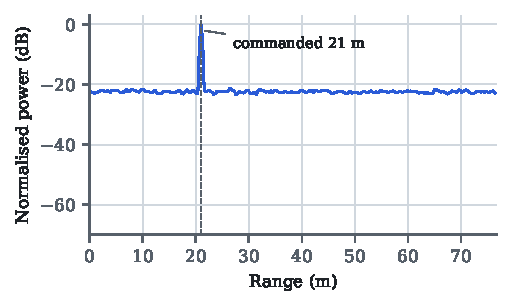
\includegraphics[width=\linewidth]{range_profile_21m.pdf}
  \caption{Range profile of one synthetic frame commanded at \SI{21}{\metre} (per-sample SNR \SI{0}{\decibel}). The peak lands on the commanded range in a single generation.}
  \label{fig:profile}
\end{figure}

\emph{Range sweep (S1).} Frames were generated for 1{,}101 ranges from \SIrange{5}{60}{\metre} in \SI{5}{\centi\metre} steps. Without noise, every estimate fell within one bin; the RMSE was \SI{0.34}{\centi\metre} and the largest error \SI{0.47}{\centi\metre}. This residual is the known bias of parabolic peak interpolation on a Hann-windowed spectrum, not a property of the generator. At \SI{0}{\decibel} per-sample SNR, the RMSE over the same sweep was \SI{0.31}{\centi\metre}.

\emph{Noise robustness.} \Cref{fig:snr} shows the range RMSE as the per-sample SNR falls from \SI{10}{\decibel} to \SI{-34}{\decibel}, using 56 ranges and five noise draws per SNR. The error stays below \SI{3}{\centi\metre} down to \SI{-22}{\decibel}, because the FFT and chirp averaging integrate the signal over \num{32768} samples. Below that the estimator breaks down quickly: \SI{99.6}{\percent} of estimates are within one bin at \SI{-24}{\decibel}, \SI{83.9}{\percent} at \SI{-26}{\decibel} and \SI{21.8}{\percent} at \SI{-30}{\decibel}, as noise peaks begin to exceed the target.

\begin{figure}[t]
  \centering
  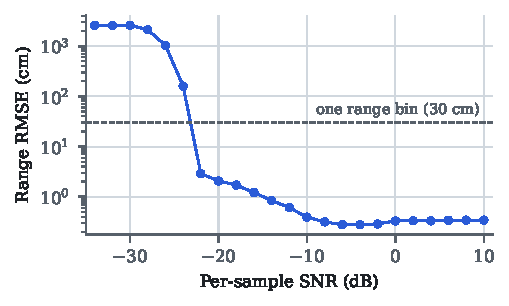
\includegraphics[width=\linewidth]{range_rmse_vs_snr.pdf}
  \caption{Range RMSE versus per-sample SNR (56 ranges from \SIrange{5}{60}{\metre}, five noise draws each). Error stays far below one range bin down to \SI{-22}{\decibel}, then breaks down within a few decibels.}
  \label{fig:snr}
\end{figure}

\Cref{tab:baseline} summarises the comparison with the brute-force approach.

\begin{table}[t]
  \centering
  \caption{Physics-based generation versus brute-force emulation}
  \label{tab:baseline}
  \footnotesize
  \begin{tabular}{@{}lll@{}}
    \toprule
    & Brute force \cite{khalil2020radar} & This work \\
    \midrule
    Attempts for \SI{21}{\metre}   & 42{,}218 & 1 \\
    Ranges reachable               & one      & any, \SIrange{5}{60}{\metre} \\
    Range error                    & not reported & \SI{0.34}{\centi\metre} RMSE \\
    Speed, target count            & fixed    & per scatterer \\
    Verification                   & closed vendor & open reference \\
    \bottomrule
  \end{tabular}
\end{table}

\subsection{Dynamic Docking (RQ2)}
\emph{Nominal docking (S3, S4).} \Cref{fig:tracks}(a) shows the nominal approach. The track starts \SI{0.4}{\second} into the run, at the third frame, and follows the truth to the stop. The track range RMSE was \SI{0.87}{\centi\metre} and the speed RMSE \SI{0.031}{\metre\per\second}. Over 20 runs with different noise seeds, the AIBT error had a mean of \SI{+0.10}{\second} and a largest magnitude of \SI{0.17}{\second}, and the reported stop position was within \SI{1.4}{\centi\metre} of the truth. In S4, with a longer and gentler deceleration, the AIBT was \SI{0.33}{\second} early in all 20 runs. The speed falls below the \SI{0.1}{\metre\per\second} stop threshold during the last moments of braking, and the logic backdates the AIBT to the start of the stationary window, so this bias follows directly from the rule and the deceleration.

\begin{figure}[t]
  \centering
  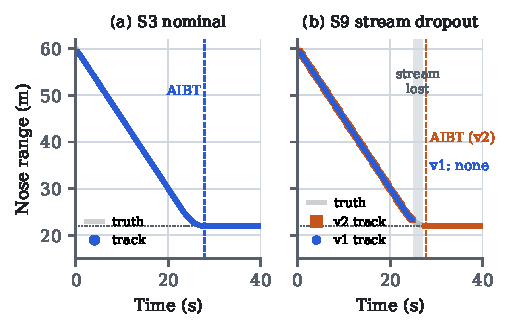
\includegraphics[width=\linewidth]{docking_tracks.pdf}
  \caption{Tracked nose range against truth. (a) Nominal docking S3; the dashed line marks the AIBT. (b) S9: the detection stream is lost for \SI{2}{\second} just before the stop. The v1 logic loses the track and never reports an AIBT; v2 re-acquires the parked aircraft and reports it.}
  \label{fig:tracks}
\end{figure}

\emph{Overshoot (S5).} With the aircraft stopping \SI{1.0}{\metre} past the line, the overshoot alarm was raised at \SI{26.8}{\second}, before the stop, and the AIBT message reported the stop \SI{1.01}{\metre} past the line.

\emph{Obstacles (S6, S7).} \Cref{fig:rdmap} shows one range--Doppler frame of S6. The crossing vehicle appears closer than the aircraft and with a different radial speed, so it is not associated with the aircraft track. In both S6 and S7, the obstacle alarm was raised in the first frame in which the vehicle or the person entered the field of view, stayed on in every frame they were visible, and never fired outside those frames. The person has an RCS of only \SI{0.5}{\square\metre}, but at about \SI{10}{\metre} the $R^{-4}$ law makes its echo stronger than that of the aircraft nose at \SI{40}{\metre}.

\begin{figure}[t]
  \centering
  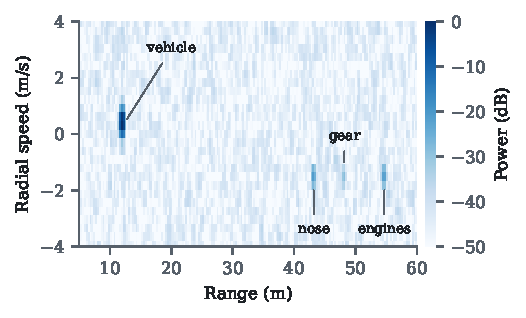
\includegraphics[width=\linewidth]{rd_map_s6.pdf}
  \caption{Range--Doppler map of one frame of S6 at \SI{11.2}{\second}. The aircraft's three scattering centres share one radial speed; the crossing vehicle is closer and moves differently.}
  \label{fig:rdmap}
\end{figure}

\emph{Degraded SNR (S8).} Fog attenuation at millimetre wavelengths over a few tens of metres is small, which is the reason radar is added. Lowering the reference SNR therefore stands for other losses, such as heavy rain, a wet or iced radome, or misalignment, and tests the margin of the processing chain. \Cref{fig:capture} shows how the capture range shrinks as the reference SNR falls, over 10 runs per level. Down to \SI{-33}{\decibel}, every run captured the aircraft and, with the v2 logic, reported a correct AIBT, but capture moved from \SI{59.4}{\metre} to a median of \SI{25.9}{\metre}, only \SI{3.9}{\metre} before the stop line. At \SI{-36}{\decibel} one run in ten captured the aircraft, and at \SI{-39}{\decibel} none did. In the single S8 run at \SI{-30}{\decibel}, only \SI{61.1}{\percent} of frames passed the sensor-level check, yet the docking itself passed, because the track did not need the aircraft until it was close.

\begin{figure}[t]
  \centering
  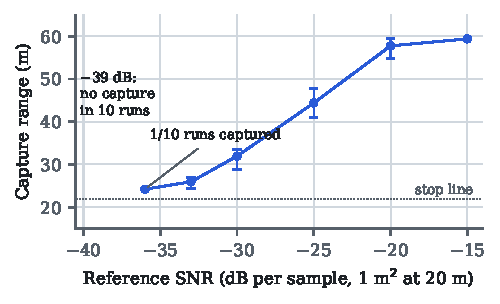
\includegraphics[width=\linewidth]{capture_vs_snr.pdf}
  \caption{Range at which the docking logic (v2) captured the aircraft versus reference SNR (median, with minimum and maximum over 10 runs). Capture moves toward the stop line as SNR falls, then fails.}
  \label{fig:capture}
\end{figure}

\subsection{Stream Faults and Integration Effects (RQ3)}
\emph{Stream dropout (S9).} When the detection stream was lost for \SI{2}{\second} during final braking, the v1 logic declared track loss after \SI{1}{\second} without messages. When messages resumed, the aircraft was almost stopped, and the capture rule only accepts approaching objects, so no new track started and no AIBT was ever reported (\cref{fig:tracks}(b)). The mock AODB therefore had no AIBT and could not compute a TOBT. The sensor-level check passed in \SI{100}{\percent} of frames, because the radar and its processing were working throughout.

\emph{Stream latency (S10).} A constant \SI{0.5}{\second} delay shifted the AIBT by the same amount when events were stamped with the receive time (\SI{+0.47}{\second} against \SI{-0.03}{\second} without delay). With sensor time stamps, the AIBT error stayed at \SI{-0.03}{\second} for every delay tested up to \SI{2}{\second}. In this run, none of the delays changed the minute-rounded TOBT. A delay $\delta$ changes the TOBT only when it moves the AIBT across a minute boundary, which for an AIBT uniformly placed within the minute happens with probability $\delta/(\SI{60}{\second})$, or \SI{3.3}{\percent} for \SI{2}{\second}.

\emph{Frozen sensor output (S13).} When the sensor repeated its last frame for \SI{3}{\second}, the track drifted from the truth, the logic lost it, and v1 again reported no AIBT. Here the sensor-level check did flag the fault, with \SI{93.4}{\percent} of frames passing.

\emph{Ghost echo (S11).} A stationary reflector of \SI{20}{\square\metre} was placed \SI{1}{\metre} short of the stop line. From \SI{24.6}{\second}, when the nose came within about two range bins of it, the nose detection disappeared: the CFAR cells around the stronger ghost connected to the nose echo, clustering merged the two, and only the ghost's peak was reported, even though the nose still moved at about \SI{1}{\metre\per\second}. The v1 logic lost the track, re-captured the nose gear \SI{5}{\metre} behind the nose, and reported an AIBT with the aircraft \SI{4.99}{\metre} short of the line. The obstacle alarm also fired in 213 frames without any real obstacle.

\emph{Sensor-level versus end-to-end.} Of the four v1 failures in \cref{tab:catalogue} (S9, S11, S12, S13), the sensor-level check flagged two (S11, S13) and missed two (S9, S12). It also flagged S8, where the docking was correct. Sensor-level checks therefore neither found all faults that reach airport operations, nor did their alarms identify which faults mattered.

\subsection{Iteration: From v1 to v2}
\label{sec:iteration}
The failures above, together with one found in the SNR sweep, led to three rules added to the docking logic, forming v2:
\begin{itemize}
  \item \emph{Re-acquisition} (from S9, S13): for \SI{10}{\second} after a track loss, a detection within \SI{2}{\metre} of the last tracked range may restart the track regardless of its speed.
  \item \emph{Nose re-selection} (from the SNR sweep): while the aircraft moves faster than \SI{0.3}{\metre\per\second}, a detection that stays more than \SI{1}{\metre} in front of the track with the same speed for three frames becomes the new track. At \SI{-20}{\decibel}, the weak nose was missed at long range and v1 captured the engine inlets in 3 of 10 runs, reporting the stop \SI{11.5}{\metre} off.
  \item \emph{AOBT backdating} (from S12): the AOBT is stamped at the last frame in which the aircraft was still within \SI{5}{\centi\metre} of its stop position.
\end{itemize}

With v2, S9 and S13 reported the AIBT within \SI{-0.03}{\second} and \SI{+0.97}{\second}, the S12 AOBT error fell from \SI{2.37}{\second} to \SI{0.57}{\second}, and every SNR level down to \SI{-33}{\decibel} gave a correct AIBT in 10 of 10 runs (v1: 7 of 10 at \SI{-20}{\decibel}, 9 of 10 at \SI{-25}{\decibel}). The nominal scenarios gave identical results under both versions. S11 still fails under v2, in a different way: the re-acquisition rule locks onto the ghost itself and reports the AIBT \SI{1.63}{\second} early with the stop \SI{1.00}{\metre} short. Each fix is now a regression test, and the ghost case is kept as a test marked as an expected failure. Overall, v1 passed 7 of the 11 end-to-end scenarios and v2 passed 10.

\subsection{Run Time}
Generating and processing one frame for the static experiments took \SI{3.4}{\milli\second} on average over 200 runs. The full pipeline, including range--Doppler processing, CFAR, JSON encoding, loopback UDP and the docking logic, took \SI{14.2}{\milli\second} per frame on average, or \SI{7}{\percent} of the \SI{200}{\milli\second} available at \SI{5}{\hertz}. The median UDP transfer took \SI{0.03}{\milli\second} for a median message size of 521 bytes. Times were measured on a single development machine and will vary with hardware.
% NOTE TO AUTHOR: rerun experiments on your own machine and add its CPU model here.

% ============================================================
\section{Discussion}
\label{sec:discussion}

\emph{What the results show.} For RQ1, the answer is clear: once the signal is modelled instead of searched for, any range is one evaluation of \cref{eq:signal} away, and the accuracy is limited by the processor, not the generator. For RQ2, the framework reproduced the docking cases that a VDGS must handle, at a cost far below the frame budget, so scenarios can run faster than real time in continuous integration. For RQ3, the most useful results are the failures. A \SI{2}{\second} gap in the detection stream left the AODB without an AIBT while every sensor-level check passed; a stationary echo moved the reported stop position by \SI{5}{\metre}; and the choice of clock for event stamps decided whether network latency reached A-CDM at all. None of these is visible when the radar is tested on its own.

\emph{Why the ghost case is still open.} The ghost failure starts in the processor, not in the docking logic. Once the nose is within about two range bins of the stationary ghost, connected-component clustering joins their CFAR cells into one cluster, and the cluster reports only the stronger ghost. Logic rules alone cannot recover a detection that was never produced. Likely fixes are local-maximum detection within clusters, a clutter map learned on the empty stand, or angle measurement with more receive channels. The framework gives a direct test for any of them.

\emph{Threats to validity.} First, the scene model is simple. Scatterers are points with fixed RCS; the real aircraft signature changes with aspect and type, and multipath, ground clutter and the terminal structure are not modelled \cite{holder2018challenges}. The results are therefore an optimistic bound on accuracy, and the aircraft profile is illustrative. Second, a lower SNR is only a proxy for adverse conditions; precipitation attenuation and radome effects are not modelled physically. Third, the radar has a single receive channel and measures no angle, so lateral position and centreline deviation are outside the scope. Fourth, the docking logic and the AODB are reference implementations. Their rules are plausible and based on published documents, but a vendor's logic may behave differently, and the specific failures found here belong to v1, not to any product. What transfers is the method: the same scenarios and faults can be run against any logic that consumes the same messages. Finally, the acceptance thresholds, such as \SI{1}{\second} for the AIBT, were chosen by the author and have not yet been reviewed by airport operators.

% ============================================================
\section{Conclusion and Future Work}
\label{sec:conclusion}
This paper presented an open framework that generates synthetic FMCW radar data for evaluating radar-augmented visual docking guidance systems, and follows that data through detection, docking logic and the hand-off of on-block events to airport operations. Compared with brute-force emulation of radar files, it reaches any commanded range in one generation with sub-centimetre error. On 13 scenarios it reproduced nominal dockings, overshoots, obstacles, degraded SNR and stream faults at a small fraction of the real-time budget. Its main value showed in the failures it exposed: four in the first version of a docking logic, of which three were fixed and locked in by regression tests, and one that points to a weakness in processing rather than logic.

Future work will add aspect-dependent aircraft signatures and ground clutter, possibly through ray tracing \cite{radarsimpy}; model several receive channels to cover lateral guidance; test fixes for the ghost case; run the scenarios against a hardware radar in the loop; and review the scenarios and acceptance criteria with airport operations and VDGS integration engineers.

% ============================================================
\bibliographystyle{IEEEtran}
\bibliography{references}

\end{document}
